% Options for packages loaded elsewhere
\PassOptionsToPackage{unicode}{hyperref}
\PassOptionsToPackage{hyphens}{url}
\PassOptionsToPackage{dvipsnames,svgnames,x11names}{xcolor}
%
\documentclass[
  12pt,
]{article}
\usepackage{amsmath,amssymb}
\usepackage{iftex}
\ifPDFTeX
  \usepackage[T1]{fontenc}
  \usepackage[utf8]{inputenc}
  \usepackage{textcomp} % provide euro and other symbols
\else % if luatex or xetex
  \usepackage{unicode-math} % this also loads fontspec
  \defaultfontfeatures{Scale=MatchLowercase}
  \defaultfontfeatures[\rmfamily]{Ligatures=TeX,Scale=1}
\fi
\usepackage{lmodern}
\ifPDFTeX\else
  % xetex/luatex font selection
  \setmainfont[]{Palatino}
  \setsansfont[]{Helvetica}
  \setmonofont[]{Menlo}
\fi
% Use upquote if available, for straight quotes in verbatim environments
\IfFileExists{upquote.sty}{\usepackage{upquote}}{}
\IfFileExists{microtype.sty}{% use microtype if available
  \usepackage[]{microtype}
  \UseMicrotypeSet[protrusion]{basicmath} % disable protrusion for tt fonts
}{}
\makeatletter
\@ifundefined{KOMAClassName}{% if non-KOMA class
  \IfFileExists{parskip.sty}{%
    \usepackage{parskip}
  }{% else
    \setlength{\parindent}{0pt}
    \setlength{\parskip}{6pt plus 2pt minus 1pt}}
}{% if KOMA class
  \KOMAoptions{parskip=half}}
\makeatother
\usepackage{xcolor}
\usepackage[margin = 1.2in]{geometry}
\usepackage{color}
\usepackage{fancyvrb}
\newcommand{\VerbBar}{|}
\newcommand{\VERB}{\Verb[commandchars=\\\{\}]}
\DefineVerbatimEnvironment{Highlighting}{Verbatim}{commandchars=\\\{\}}
% Add ',fontsize=\small' for more characters per line
\newenvironment{Shaded}{}{}
\newcommand{\AlertTok}[1]{\textcolor[rgb]{1.00,0.00,0.00}{\textbf{#1}}}
\newcommand{\AnnotationTok}[1]{\textcolor[rgb]{0.38,0.63,0.69}{\textbf{\textit{#1}}}}
\newcommand{\AttributeTok}[1]{\textcolor[rgb]{0.49,0.56,0.16}{#1}}
\newcommand{\BaseNTok}[1]{\textcolor[rgb]{0.25,0.63,0.44}{#1}}
\newcommand{\BuiltInTok}[1]{\textcolor[rgb]{0.00,0.50,0.00}{#1}}
\newcommand{\CharTok}[1]{\textcolor[rgb]{0.25,0.44,0.63}{#1}}
\newcommand{\CommentTok}[1]{\textcolor[rgb]{0.38,0.63,0.69}{\textit{#1}}}
\newcommand{\CommentVarTok}[1]{\textcolor[rgb]{0.38,0.63,0.69}{\textbf{\textit{#1}}}}
\newcommand{\ConstantTok}[1]{\textcolor[rgb]{0.53,0.00,0.00}{#1}}
\newcommand{\ControlFlowTok}[1]{\textcolor[rgb]{0.00,0.44,0.13}{\textbf{#1}}}
\newcommand{\DataTypeTok}[1]{\textcolor[rgb]{0.56,0.13,0.00}{#1}}
\newcommand{\DecValTok}[1]{\textcolor[rgb]{0.25,0.63,0.44}{#1}}
\newcommand{\DocumentationTok}[1]{\textcolor[rgb]{0.73,0.13,0.13}{\textit{#1}}}
\newcommand{\ErrorTok}[1]{\textcolor[rgb]{1.00,0.00,0.00}{\textbf{#1}}}
\newcommand{\ExtensionTok}[1]{#1}
\newcommand{\FloatTok}[1]{\textcolor[rgb]{0.25,0.63,0.44}{#1}}
\newcommand{\FunctionTok}[1]{\textcolor[rgb]{0.02,0.16,0.49}{#1}}
\newcommand{\ImportTok}[1]{\textcolor[rgb]{0.00,0.50,0.00}{\textbf{#1}}}
\newcommand{\InformationTok}[1]{\textcolor[rgb]{0.38,0.63,0.69}{\textbf{\textit{#1}}}}
\newcommand{\KeywordTok}[1]{\textcolor[rgb]{0.00,0.44,0.13}{\textbf{#1}}}
\newcommand{\NormalTok}[1]{#1}
\newcommand{\OperatorTok}[1]{\textcolor[rgb]{0.40,0.40,0.40}{#1}}
\newcommand{\OtherTok}[1]{\textcolor[rgb]{0.00,0.44,0.13}{#1}}
\newcommand{\PreprocessorTok}[1]{\textcolor[rgb]{0.74,0.48,0.00}{#1}}
\newcommand{\RegionMarkerTok}[1]{#1}
\newcommand{\SpecialCharTok}[1]{\textcolor[rgb]{0.25,0.44,0.63}{#1}}
\newcommand{\SpecialStringTok}[1]{\textcolor[rgb]{0.73,0.40,0.53}{#1}}
\newcommand{\StringTok}[1]{\textcolor[rgb]{0.25,0.44,0.63}{#1}}
\newcommand{\VariableTok}[1]{\textcolor[rgb]{0.10,0.09,0.49}{#1}}
\newcommand{\VerbatimStringTok}[1]{\textcolor[rgb]{0.25,0.44,0.63}{#1}}
\newcommand{\WarningTok}[1]{\textcolor[rgb]{0.38,0.63,0.69}{\textbf{\textit{#1}}}}
\usepackage{graphicx}
\makeatletter
\def\maxwidth{\ifdim\Gin@nat@width>\linewidth\linewidth\else\Gin@nat@width\fi}
\def\maxheight{\ifdim\Gin@nat@height>\textheight\textheight\else\Gin@nat@height\fi}
\makeatother
% Scale images if necessary, so that they will not overflow the page
% margins by default, and it is still possible to overwrite the defaults
% using explicit options in \includegraphics[width, height, ...]{}
\setkeys{Gin}{width=\maxwidth,height=\maxheight,keepaspectratio}
% Set default figure placement to htbp
\makeatletter
\def\fps@figure{htbp}
\makeatother
\setlength{\emergencystretch}{3em} % prevent overfull lines
\providecommand{\tightlist}{%
  \setlength{\itemsep}{0pt}\setlength{\parskip}{0pt}}
\setcounter{secnumdepth}{5}
\newlength{\cslhangindent}
\setlength{\cslhangindent}{1.5em}
\newlength{\csllabelwidth}
\setlength{\csllabelwidth}{3em}
\newlength{\cslentryspacingunit} % times entry-spacing
\setlength{\cslentryspacingunit}{\parskip}
\newenvironment{CSLReferences}[2] % #1 hanging-ident, #2 entry spacing
 {% don't indent paragraphs
  \setlength{\parindent}{0pt}
  % turn on hanging indent if param 1 is 1
  \ifodd #1
  \let\oldpar\par
  \def\par{\hangindent=\cslhangindent\oldpar}
  \fi
  % set entry spacing
  \setlength{\parskip}{#2\cslentryspacingunit}
 }%
 {}
\usepackage{calc}
\newcommand{\CSLBlock}[1]{#1\hfill\break}
\newcommand{\CSLLeftMargin}[1]{\parbox[t]{\csllabelwidth}{#1}}
\newcommand{\CSLRightInline}[1]{\parbox[t]{\linewidth - \csllabelwidth}{#1}\break}
\newcommand{\CSLIndent}[1]{\hspace{\cslhangindent}#1}
\ifLuaTeX
\usepackage[bidi=basic]{babel}
\else
\usepackage[bidi=default]{babel}
\fi
\babelprovide[main,import]{french}
\ifPDFTeX
\else
\babelfont[french]{rm}[]{Palatino}
\fi
% get rid of language-specific shorthands (see #6817):
\let\LanguageShortHands\languageshorthands
\def\languageshorthands#1{}
\ifLuaTeX
  \usepackage{selnolig}  % disable illegal ligatures
\fi
\IfFileExists{bookmark.sty}{\usepackage{bookmark}}{\usepackage{hyperref}}
\IfFileExists{xurl.sty}{\usepackage{xurl}}{} % add URL line breaks if available
\urlstyle{same}
\hypersetup{
  pdftitle={PSTL : Interface Web Autobill},
  pdfauthor={Fazazi Zeid; Luo Yukai; Dibassi Brahima},
  pdflang={fr},
  colorlinks=true,
  linkcolor={Maroon},
  filecolor={Maroon},
  citecolor={Blue},
  urlcolor={NavyBlue},
  pdfcreator={LaTeX via pandoc}}

\title{PSTL : Interface Web Autobill}
\usepackage{etoolbox}
\makeatletter
\providecommand{\subtitle}[1]{% add subtitle to \maketitle
  \apptocmd{\@title}{\par {\large #1 \par}}{}{}
}
\makeatother
\subtitle{Pré-Rapport}
\author{Fazazi Zeid \and Luo Yukai \and Dibassi Brahima}
\date{2023-04-11}

\begin{document}
\maketitle

\textbf{Encadrants : Hector Suzanne, Emmanuel Chailloux} \newpage

{
\hypersetup{linkcolor=}
\setcounter{tocdepth}{3}
\tableofcontents
}
\newpage

\hypertarget{contexte-du-projet}{%
\section{Contexte du projet}\label{contexte-du-projet}}

\hypertarget{historique-et-duxe9finitions}{%
\subsection{Historique et
définitions}\label{historique-et-duxe9finitions}}

\href{https://gitlab.lip6.fr/suzanneh/autobill}{\textbf{Autobill}} est
un projet universitaire développé par notre tuteur de projet Hector
Suzanne, au sein de l'équipe APR du LIP6, dans le cadre de sa thèse sur
l'analyse statique de la consommation mémoire d'un programme.

L'analyse statique est un domaine de l'informatique qui consiste à
mesureer et détecter automatiquement les comportements ou erreurs dans
un programme en examinant son code source. Pour effectuer cette analyse
sur un langage de programmation donné, il est possible de définir des
règles d'évaluation et de typage. Dans notre situation spécifique, nous
sommes particulièrement intéressés par l'occupation de la mémoire d'un
programme.

Historiquement, ce sujet de recherche a été plusieurs fois abordé dans
divers travaux scientifiques, parmi eux, ceux de Jan Hoffmann sur
l'analyse de consommation de ressources automatisé
\protect\hyperlink{ref-Hoffmann}{{[}1{]}}. Des solutions se basant sur
ces théories existent, comme RAML \protect\hyperlink{biblio}{{[}2{]}}
(Resource Aware ML), un langage \emph{à la ML} permettant ce type
d'analyse, créé par Jan Hoffman et Stephen Jost.

\hypertarget{quest-ce-quautobill}{%
\subsection{Qu'est-ce qu'Autobill ?}\label{quest-ce-quautobill}}

La proposition d'Hector Suzanne avec Autobill se différencie par un
niveau d'analyse plus précis sur les fermetures et les arguments
fonctionnels d'un programme. D'abord, Autobill prend en entrée des
programmes écrits soit en modèle machine propre à Autobill, soit en
\textbf{Call-By-Push-Value} (CBPV), avec ou sans continuation explicite.

C'est un langage qui utilise un paradigme déjà éprouvé, décrit dans la
thèse de Paul Blain Lévy \protect\hyperlink{biblio}{{[}3{]}}. CBPV
utilise une pile pour stocker les valeurs et les fonctions manipulées
dans le programme. Ainsi, on peut suivre de manière explicite les
quantités de mémoire pour chaque valeur introduite/éliminée ou fonction
appelée/terminée. Aussi, le langage permet d'exprimer clairement les
stratégies d'évaluation utilisées dans le code source : on fixe quand
les évaluations se déroulent, afin de mieux prédire la consommation de
mémoire à chaque étape du programme.

À partir d'une entrée en CBPV, Autobill traduit le programme en un code
machine avec continuation, exprimant explicitement les contraintes de
taille qui s'appliquent sur l'entrée. Il l'internalise, c'est à dire
construit l'arbre syntaxique abstrait (AST) de ce programme. Ensuite,
Autobill infère dans l'AST le typage de ses expressions ainsi que leurs
polarités. Enfin, il en tire en sortie les contraintes dans des formats
d'entrées supportés par différents outils de recherche opérationnelles
et assistants de preuve, comme
\href{https://www.minizinc.org/}{MiniZinc} ou
\href{https://coq.inria.fr/}{Coq}, afin de prouver des propriétés de
complexité temporelle ou spatiale.

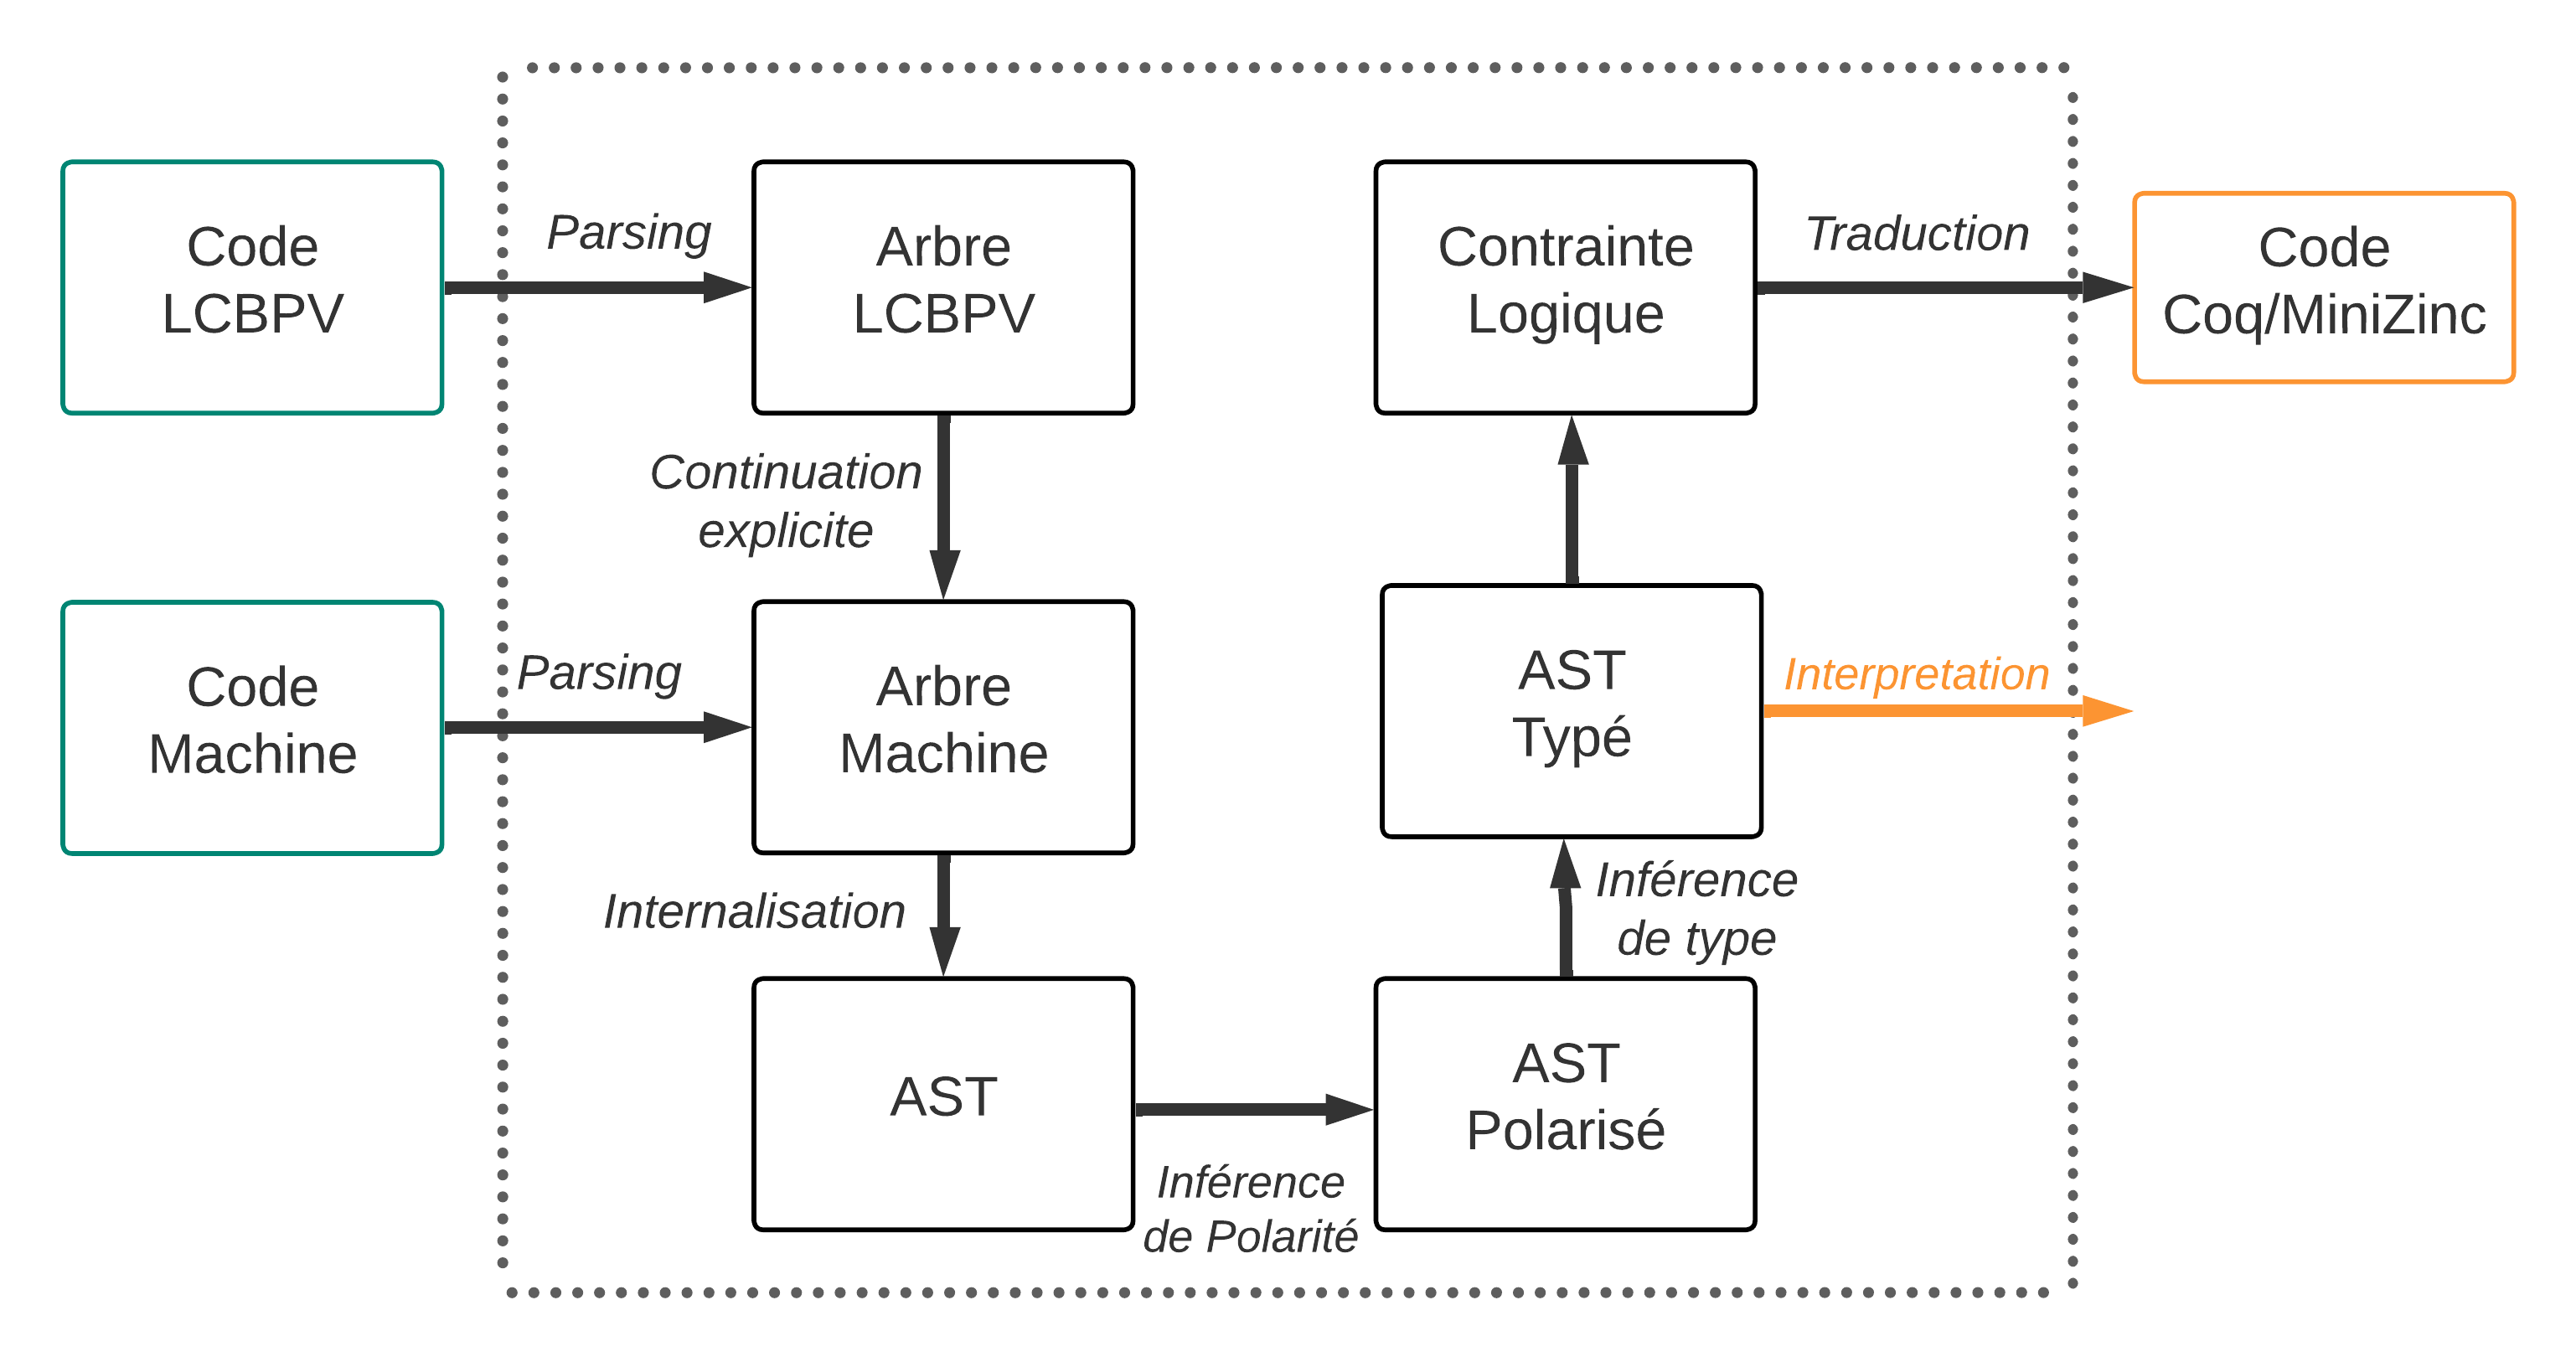
\includegraphics{./MarkdownVersions/Rapport/Schema_Autobill.png}

\hypertarget{objectifs-du-projet}{%
\subsection{Objectifs du projet}\label{objectifs-du-projet}}

Notre démarche se rapproche de celle de RAML
\protect\hyperlink{biblio}{{[}2{]}} dans leur site officiel.

Le sujet de notre projet STL va donc être de soutenir l'effort de
développement en proposant une interface sur le Web permettant la libre
manipulation de l'outil Autobill par des utilisateurs à travers un
environnement de développement sur navigateur.

On souhaite aussi faciliter l'utilisation de l'outil avec un langage
fonctionnel pur en entrée plus accessible, un \textbf{MiniML}. Cela nous
contraint donc à adapter cette nouvelle entrée pour qu'elle soit
compatible avec Autobill. Enfin, on se charge aussi de traiter les
différentes sorties standards et d'erreurs d'Autobill, notamment les
expressions de contraintes, afin de les passer à des solveurs externes,
en tirer des preuves de complexité et les afficher directement sur le
client Web.

Notre charge de travail doit se diviser en plusieurs tâches principales
:

\begin{itemize}
\tightlist
\item
  L'implémentation du langage MiniML et sa traduction vers LCBPV
\item
  La mise en place d'une interface Web
\item
  La mise en relation entre l'interface Web et la machine Autobill
\item
  Le traitement des contraintes d'Autobill par un solveur externe
\item
  Les tests de performances et comparaisons avec les solutions
  existantes
\end{itemize}

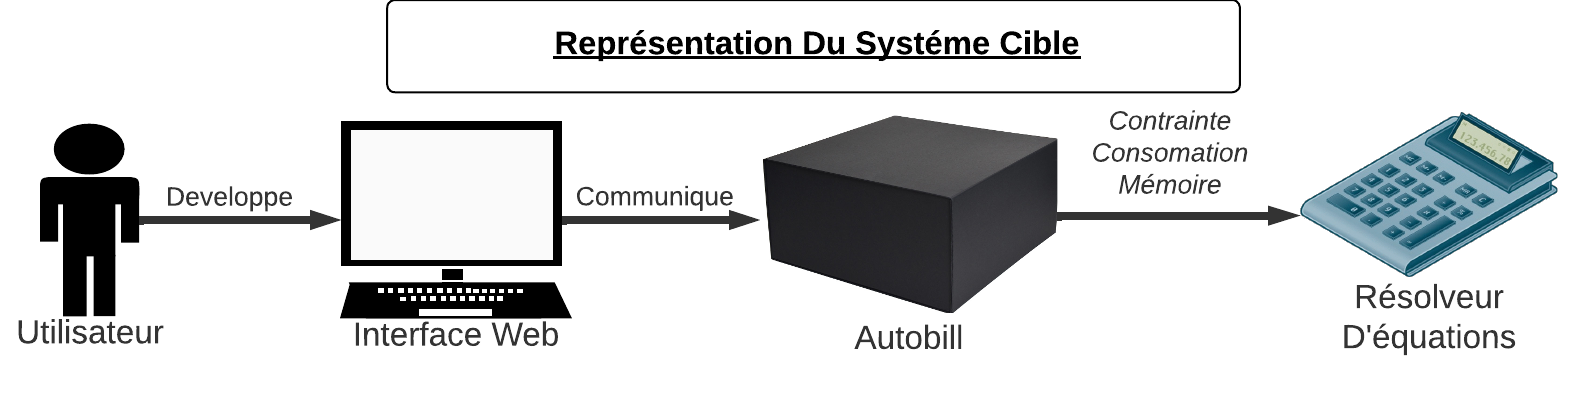
\includegraphics{./MarkdownVersions/Rapport/Diagramme Haut Niveau PSTL.png}

\hypertarget{processus-de-conception}{%
\subsection{Processus de conception}\label{processus-de-conception}}

Lors de la conception de l'interface, les contraintes étaient multiples.
La première était l'interopérabilité des technologies du projet. En
effet \textbf{Autobill} étant développé en \textbf{OCaml}, il était
nécessaire de trouver des moyens pour l'adapter à un environnement
Web.La seconde était qu'il fallait développer cette interface en
simultané avec \textbf{Autobill} et ajuster notre travail en fonction
des besoins courants de nos encadrants.Mais la plus importante d'entre
elles était le souhait de nos encadrants que l'application soit
principalement côté client afin de simplifier son déploiement dans les
infrastructures de la faculté.

Une fois ces contraintes établies, nous avons dû,tout au long de ce
projet, effectuer des choix, que ce soit en matière de design ou de
technologies.Nous tenons donc à travers ce rapport à mettre en lumière
ces décisions, tout en décrivant le travail qu'elles ont engendré.

\newpage

\hypertarget{interface-web}{%
\section{Interface web}\label{interface-web}}

Dans l'optique de ne pas se restreindre dans l'utilisation d'outils
notamment au niveau du résolveur de contraintes, le groupe s'est orienté
vers deux structures de projets différentes et indépendantes : l'une
fonctionnant avec un client unique, la seconde avec un serveur dédié et
un client qui expose ce serveur.

L'avantage réside dans le fait que, lors du développement, si un nouvel
outil est amené à être utilisé mais ne dispose de compatibilité sur
navigateur Web, alors le serveur peut répondre à ce problème. C'est
aussi un sujet de comparaison intéressant à présenter par la suite, que
ce soit au niveau des performances que du déploiement de ces solutions.

\hypertarget{client-uniquement}{%
\subsection{Client uniquement}\label{client-uniquement}}

\hypertarget{outils-et-technologies-utilisuxe9s}{%
\subsubsection{Outils et Technologies
utilisés}\label{outils-et-technologies-utilisuxe9s}}

\begin{itemize}
\item
  \textbf{HTML / CSS / Javascript (JS)} : Il s'agit de la suite de
  langages principaux permettant de bâtir l'interface Web souhaitée. On
  a ainsi la main sur la structure de la page à l'aide des balises HTML,
  du style souhaité pour l'éditeur de code avec le CSS et on vient
  apporter l'interactivité et les fonctionnalités en les programmant
  avec Javascript, complété par la librairie React.
\item
  \textbf{React.js} : React.js est une bibliothèque JavaScript
  open-source pour la création d'interfaces utilisateur,utilisée pour la
  création d'applications web modernes et interactives. Parmi les
  avantages de cette technologie, il y a l'utilisation du Virtual DOM
  (Document Object Model) qui permet une mise à jour plus efficace et
  rapide des éléments d'une page. Le Virtual DOM est une représentation
  virtuelle d'un arbre DOM qui est stockée en mémoire et mise à jour en
  temps réel en fonction des interactions de l'utilisateur avec
  l'interface. On modifie seulement les éléments impactés, et non
  l'ensemble du DOM de la page, ce qui se traduit par des temps de
  réponse plus rapides et des meilleures performances. Aussi, React est
  basé sur la programmation orientée composant. L'interface utilisateur
  est décomposée en petits composants réutilisables, chacun étant
  responsable de l'affichage d'une partie spécifique de l'interface.
  Chaque composant est construit de manière indépendante et peut être
  utilisé à plusieurs endroits dans une application. Cette approche
  modulaire rend l'interface plus flexible et maintenable.
\item
  \textbf{CodeMirror} : C'est une librairie Javascript permettant
  d'intégrer un éditeur de code puissant, incluant le support de la
  coloration syntaxique, de l'autocomplétion ou encore le surlignage
  d'erreurs. Les fonctionnalités de l'éditeur sont grandement extensives
  et permettant même la compatibilité avec un langage de programmation
  personnalisé comme \textbf{MiniML}. Enfin, CodeMirror est disponible
  sous licence MIT, libre de droits.
\end{itemize}

\newpage

\begin{itemize}
\item
  \textbf{OCaml + Js\_of\_OCaml} : Afin de manipuler la librairie
  d'\textbf{Autobill}, il est nécessaire de passer par du côté OCaml
  pour traiter le code en entrée et en sortir des équations à résoudre
  ou des résultats d'interprétations. Pour faire le pont entre
  Javascript et OCaml, on utilise Js\_of\_OCaml, une librairie
  contenant, entre autres, un compilateur qui transpile du bytecode
  OCaml en Javascript et propose une grande variété de primitive et de
  type pour manipuler des éléments Javascript depuis OCaml. L'API de
  Js\_of\_Ocaml est suffisamment fournie pour développer entièrement des
  applications web complètes et fonctionnelles. Pour ce projet, il sert
  surtout pour interagir avec Autobill et la librairie de MiniML depuis
  le client Web. Dans un fichier \texttt{main.ml}, on exporte un objet
  Javascript contenant plusieurs méthodes correspondant chacune à un
  mode d'exécution différent d'Autobill. Chaque méthode prend en entrée
  le code MiniML à traiter et réalise les transformations nécessaires
  pour générer la sortie demandée. Néanmoins, en l'absence de sortie
  standard ou d'erreurs, les messages d'exceptions d'Ocaml, par exemple,
  n'apparaissent que dans la console Javascript du navigateur.
  Js\_of\_ocaml met à notre disposition un module \texttt{Sys\_js} qui
  offre des primitives permettant de capturer les possibles messages sur
  les sorties et les rediriger dans des buffers. Ces buffers peuvent
  être convertis en chaînes de caractères et retournés au client par la
  suite.
\item
  \textbf{MiniZinc}: À la génération des expressions de contraintes,
  Autobill retourne une sortie au format MiniZinc. Ce langage permet de
  décrire des problèmes de manière déclarative à l'aide de contraintes
  logiques. L'objectif avec MiniZinc est de calculer les bornes mémoires
  minimums pour satisfaire les contraintes mémoires du programme et
  d'afficher, sous forme d'équation, le résultat dans la sortie de notre
  IDE. Son API prend en charge une large gamme de solveurs. Aussi, il
  dispose d'une grande communauté d'utilisateurs et de contributeurs, ce
  qui nous permet de trouver nombreuses ressources disponibles pour
  l'apprentissage et le dépannage. Sa librairie est codée en C++ mais il
  reste utilisable dans notre interface Web grâce à Web Assembly. C'est
  un format binaire de code exécutable qui permet de porter des
  applications codées dans des langages de programmation sur le Web.
  Grâce à des compilateurs vers Web Assembly, comme Emscripten pour
  C/C++, on peut lancer des tâches intensives de résolution de
  contraintes, avec des performances proches du natif, depuis n'importe
  quel navigateur Web moderne.
\end{itemize}

\hypertarget{aperuxe7u-de-linterface-graphique}{%
\subsubsection{Aperçu de l'interface
graphique}\label{aperuxe7u-de-linterface-graphique}}

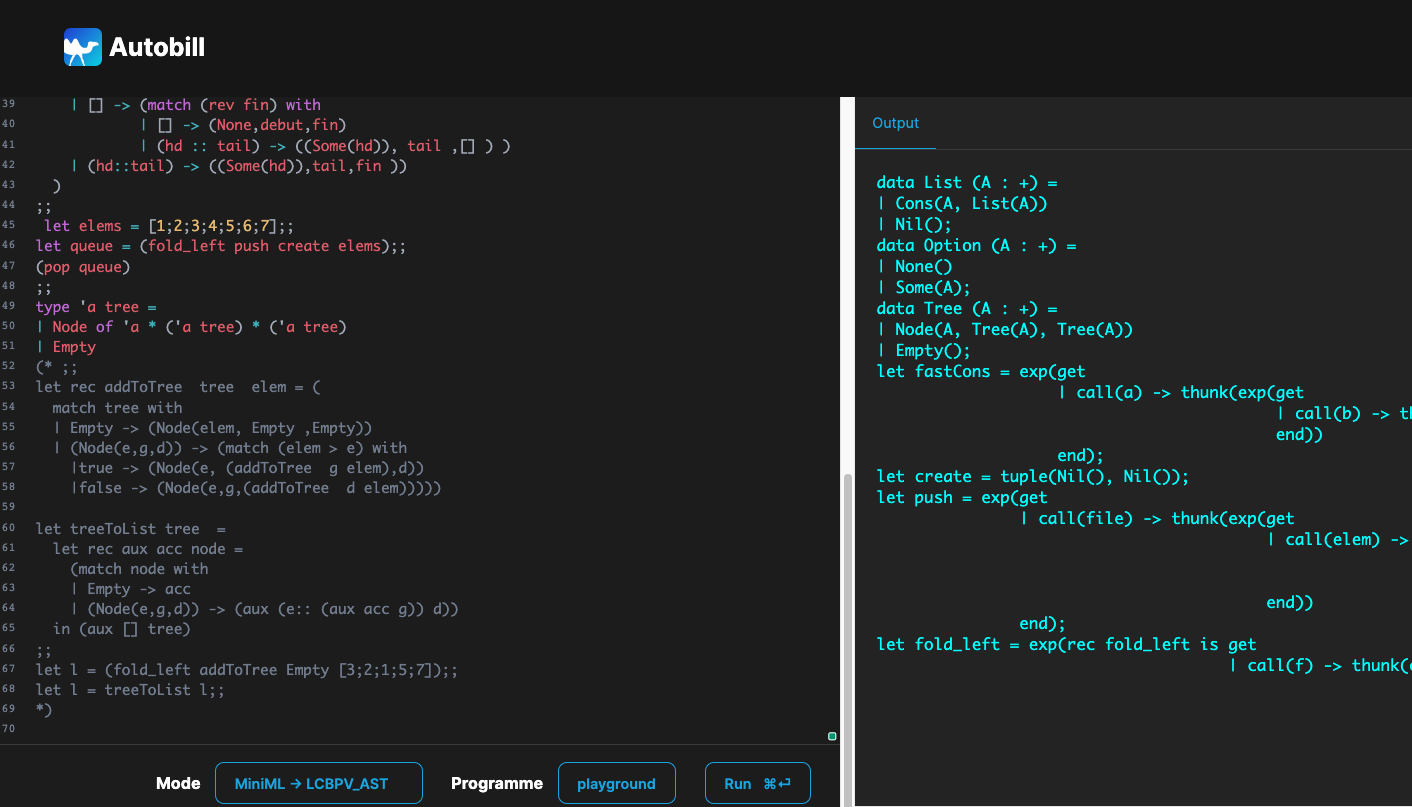
\includegraphics{./MarkdownVersions/Rapport/screen.png}

\hypertarget{tuxe2ches-ruxe9alisuxe9es}{%
\subsubsection{Tâches réalisées}\label{tuxe2ches-ruxe9alisuxe9es}}

\begin{itemize}
\tightlist
\item
  Intégration d'un IDE similaire aux \emph{Playground} de
  \href{https://OCaml.org/play}{OCaml} et
  \href{https://rescript-lang.org/try}{Rescript}
\item
  Implémentation d'un éditeur de code supportant la syntaxe de
  \textbf{MiniML}
\item
  Liaison entre le code Javascript et OCaml à l'aide de Js\_of\_OCaml
\item
  Implémentation de plusieurs modes de traitement du code
  \textbf{MiniML} :

  \begin{itemize}
  \tightlist
  \item
    Affichage de l'AST MiniML
  \item
    Affichage de l'AST de \textbf{Call-By-Push-Value}
  \item
    Affichage de l'équation résultant de l'analyse statique
  \item
    Vers Représentation Interne \textbf{Autobill}
  \end{itemize}
\item
  Remontée d'erreurs et affichage dynamique sur l'interface
\item
  Implémentation du solveur d'équations MiniZinc côté client
\end{itemize}

\hypertarget{serveur-client}{%
\subsection{Serveur + client}\label{serveur-client}}

\hypertarget{schuxe9ma-de-communication}{%
\subsubsection{Schéma de
communication}\label{schuxe9ma-de-communication}}

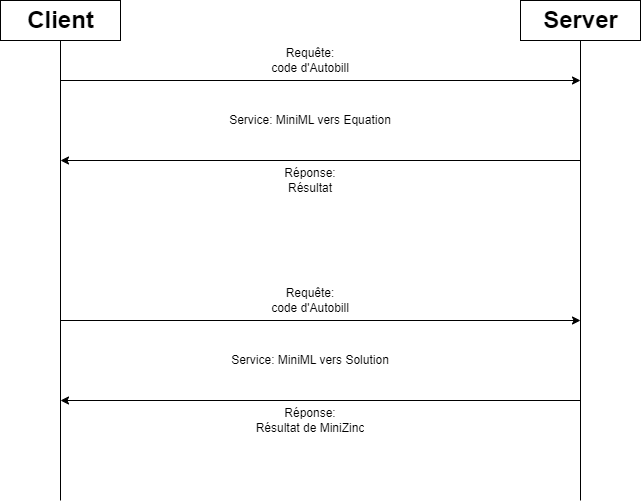
\includegraphics{./MarkdownVersions/Rapport/communication.png}

\hypertarget{outils-et-technologies-utilisuxe9s-1}{%
\subsubsection{Outils et technologies
utilisés}\label{outils-et-technologies-utilisuxe9s-1}}

\hypertarget{cotuxe9-client}{%
\paragraph{Coté client}\label{cotuxe9-client}}

\begin{itemize}
\tightlist
\item
  \textbf{HTML / CSS / Javascript}
\item
  \textbf{React.js}
\item
  \textbf{CodeMirror}
\item
  \textbf{OCaml + Js\_of\_OCaml}
\item
  \textbf{MiniZinc}
\end{itemize}

\hypertarget{cotuxe9-serveur}{%
\paragraph{Coté serveur}\label{cotuxe9-serveur}}

\begin{itemize}
\tightlist
\item
  \textbf{NodeJS}: NodeJS permet une gestion asynchrone des opérations
  entrantes, ce qui permet d'exécuter plusieurs opérations simultanément
  sans bloquer le fil d'exécution principal. Par exemple, si deux
  requête sont envoyé au serveur en même temps, elles seront gérées en
  parallèle par le serveur. Ainsi, grâce à cette gestion asynchrone,
  NodeJS permet d'optimiser l'utilisation des ressources système en
  réduisant les temps d'attente et en évitant les blocages inutiles, ce
  qui peut augmenter l'efficacité et les performances du programme. En
  outre, NodeJS est également connu pour son excellent support de la
  gestion des entrées/sorties et du traitement de données en temps réel.
  Enfin, la grande quantité de packages disponible sur NPM (le
  gestionnaire de packages de Node Js) permet de gagner beaucoup de
  temps de développement et de faciliter notre tâche. Par example, le
  module \href{https://nodejs.org/api/child_process.html}{``Child
  Processes''} nous permet d'exécuter le code MiniZinc en passant les
  commandes directement. Cela nous permet d'éviter les restrictions du
  côté full-client au niveau du résolveur de contraintes.
\end{itemize}

\hypertarget{tuxe2ches-ruxe9alisuxe9es-1}{%
\subsubsection{Tâches réalisées}\label{tuxe2ches-ruxe9alisuxe9es-1}}

\begin{itemize}
\tightlist
\item
  Intégration d'une IDE similaire aux Playground de
  \href{https://OCaml.org/play}{OCaml} et
  \href{https://rescript-lang.org/try}{Rescript}
\item
  Implémentation d'un éditeur de code supportant la syntaxe de
  \textbf{MiniML}
\item
  Liaison entre le code Javascript et OCaml à l'aide de Js\_of\_OCaml
\item
  Implémentation de plusieurs modes de traitement du code
  \textbf{MiniML} :

  \begin{itemize}
  \tightlist
  \item
    Affichage de l'équation résultant de l'anlyse statique
  \end{itemize}
\item
  Implémentation du solveur d'équations MiniZinc côté client et server
\end{itemize}

\hypertarget{miniml}{%
\section{MiniML}\label{miniml}}

\hypertarget{pourquoi-miniml}{%
\subsection{Pourquoi MiniML ?}\label{pourquoi-miniml}}

MiniML émerge de la volonté de créer un langage fonctionnel simple,
accessible et sans effets de bord pour les utilisateurs
d'\textbf{Autobill} car celui-ci requiert une connaissance approfondie
de la théorie autour des différentes sémantiques d'évaluation afin de
pouvoir manipuler son entrée en \textbf{Call-By-Push-Value}.

\hypertarget{call-by-push-value}{%
\subsubsection{Call-By-Push-Value}\label{call-by-push-value}}

Le paradigme de traitement de langage \textbf{Call-By-Push-Value}
utilisé par \textbf{Autobill} permet à l'aide d'une seule sémantique de
traiter deux types de stratégies d'évaluation différentes \textbf{Call
By Value} utilisée par \textbf{OCaml} et \textbf{Call By Name} utilisée
par \textbf{Haskell} pour mettre en place l'évaluation \emph{Lazy}. La
différenciation entre ces deux types de stratégies s'effectue lors de la
traduction depuis le langage d'origine.

\hypertarget{description-rapide}{%
\subsection{Description rapide}\label{description-rapide}}

\textbf{MiniML} dans ce projet dispose d'une implémentation écrite en
\textbf{OCaml}. De plus tout code \textbf{MiniML} est parfaitement
compatible avec un parseur ou compilateur \textbf{OCaml}.

\hypertarget{contenu-actuel}{%
\subsubsection{Contenu actuel}\label{contenu-actuel}}

\begin{itemize}
\tightlist
\item
  Integer
\item
  Boolean
\item
  Listes
\item
  Fonction Récusives
\item
  Opérateurs de Bases
\item
  Construction de Types de Données
\item
  Types de Données Paramétrés
\item
  Types de Données Récursifs
\item
  Variables Globales/Locales
\item
  Files \emph{(FIFO)}
\end{itemize}

\hypertarget{duxe9pendances}{%
\subsubsection{Dépendances}\label{duxe9pendances}}

\begin{itemize}
\tightlist
\item
  \textbf{Menhir} :
  \href{http://gallium.inria.fr/~fpottier/menhir/}{\emph{Menhir}} est
  l'unique dépendance de l'implémentation de \textbf{MiniML}, Cette
  librairie permet la génération d'analyseurs syntaxiques en OCaml nous
  permettant d'éviter le développement d'un analyseur syntaxique rigide.
  Cette décision compatible avec les deux architectures du projet, nous
  a permis d'économiser en temps de développement et gagné en
  flexibilité.\\
  Menhir est disponible sous licence GPL
\end{itemize}

\hypertarget{un-exemple-de-code-miniml}{%
\subsection{Un exemple de code MiniML}\label{un-exemple-de-code-miniml}}

Cet exemple de code \textbf{MiniML} est une implémentation possible
d'une file d'attente sans effet de bord en \textbf{MiniML}.

\begin{Shaded}
\begin{Highlighting}[]
  \KeywordTok{type}\NormalTok{ \textquotesingle{}a }\DataTypeTok{option}\NormalTok{ =}
\NormalTok{  | }\DataTypeTok{None}
\NormalTok{  | }\DataTypeTok{Some} \KeywordTok{of}\NormalTok{ \textquotesingle{}a}
\NormalTok{  ;;}

  \KeywordTok{let}\NormalTok{ createQueue = ([],[]);;}

  \KeywordTok{let}\NormalTok{ push file elem = }
\NormalTok{  (}\KeywordTok{match}\NormalTok{ file }\KeywordTok{with}
\NormalTok{  | (a,b) {-}\textgreater{} (a,(elem::b)))}
\NormalTok{  ;;}

  \KeywordTok{let}\NormalTok{ pop file =}
\NormalTok{    (}\KeywordTok{match}\NormalTok{ file }\KeywordTok{with}
\NormalTok{    | (debut, fin) {-}\textgreater{} }
\NormalTok{      (}\KeywordTok{match}\NormalTok{ debut }\KeywordTok{with}
\NormalTok{      | [] {-}\textgreater{} (}
                \KeywordTok{match}\NormalTok{ (rev fin) }\KeywordTok{with}
\NormalTok{                | [] {-}\textgreater{} (}\DataTypeTok{None}\NormalTok{,debut,fin)}
\NormalTok{                | (hd :: tail) {-}\textgreater{} ((}\DataTypeTok{Some}\NormalTok{(hd)), tail ,[])}
\NormalTok{              )}
\NormalTok{      | (hd::tail) {-}\textgreater{} ((}\DataTypeTok{Some}\NormalTok{(hd)),tail,fin ))}
\NormalTok{    )}
\NormalTok{  ;;}

  \KeywordTok{let}\NormalTok{ elems = [}\DecValTok{1}\NormalTok{;}\DecValTok{2}\NormalTok{;}\DecValTok{3}\NormalTok{;}\DecValTok{4}\NormalTok{;}\DecValTok{5}\NormalTok{;}\DecValTok{6}\NormalTok{;}\DecValTok{7}\NormalTok{];;}
  \KeywordTok{let}\NormalTok{ queue = (fold\_left push createFile elems);;}
\NormalTok{  (pop queue)}
\end{Highlighting}
\end{Shaded}

\hypertarget{schema-de-traduction}{%
\subsubsection{Schema de traduction}\label{schema-de-traduction}}

Dans le prochain rapport, nous allons nous baser sur une variante de cet
exemple pour décrire, avec des schémas de traduction comment l'on passe
de \textbf{MiniML} à \textbf{Call-By-Push-Value} compatible pour
\textbf{Autobill}.

\hypertarget{conclusion-et-tuxe2ches-uxe0-ruxe9aliser}{%
\section{Conclusion et tâches à
réaliser}\label{conclusion-et-tuxe2ches-uxe0-ruxe9aliser}}

\hypertarget{conclusion}{%
\subsection{Conclusion}\label{conclusion}}

La réalisation de cette interface a fait intervenir un large panel de
sujets en lien avec la formation du Master d'informatique STL et mis à
profit les connaissances acquises lors de ce semestre. Le projet est à
un stade d'avancement satisfaisant. Autobill étant encore en phase
expérimentale, celui-ci ajoute contiuellement des nouveautés et
corrections que l'on doit intégrer.

La suite consistera surtout à consolider les bases établies sur tous les
aspects du projet présentés dans ce rapport et les adapter aux
changements d'Autobill. Aussi, il serait intéressant à titre de
démonstration de comparer notre solution avec celle de Jan Hoffmann et
l'interface de RAML {[}3{]}, mentionnée en section 1.

\hypertarget{miniml-1}{%
\subsection{MiniML}\label{miniml-1}}

\begin{itemize}
\tightlist
\item
  Ajout de sucre syntaxique. (Records, Operateurs Infixes, \ldots)
\item
  Ajout d'une librairie standard.
\item
  Spécification complète du langage.
\item
  Bibliothèque de structures de données complexes
\item
  Régles de traduction de \textbf{MiniML} vers \textbf{Autobill}
\item
  Schemas de traduction d'une structure \emph{FIFO} vers
  \textbf{Autobill}
\end{itemize}

\hypertarget{serveur}{%
\subsection{Serveur}\label{serveur}}

\begin{itemize}
\tightlist
\item
  Affichage des erreurs
\item
  Réalisation des autres services pour MiniML
\item
  Réalisation de génération de solution depuis le code Autobill
\end{itemize}

\hypertarget{client}{%
\subsection{Client}\label{client}}

\begin{itemize}
\tightlist
\item
  Retouches esthétiques
\item
  Affichage des erreurs sur plusieurs lignes
\item
  Couverture d'erreurs à traiter la plus grande possible, afin d'éviter
  les blocages du client
\item
  ``Benchmark'' la résolution d'équations plus complexes avec le
  MiniZinc client
\item
  Proposer des programmes d'exemples à lancer, demandant des lourdes
  allocations mémoires.
\end{itemize}

\hypertarget{tests}{%
\subsection{Tests}\label{tests}}

\begin{itemize}
\tightlist
\item
  Comparaison d'architectures Full-Client vs Client-Serveur
\item
  Comparaison \textbf{RAML} vs \textbf{Autobill}
\end{itemize}

\newpage

\hypertarget{bibliography}{%
\section*{Bibliographie}\label{bibliography}}
\addcontentsline{toc}{section}{Bibliographie}

\hypertarget{refs}{}
\begin{CSLReferences}{0}{0}
\leavevmode\vadjust pre{\hypertarget{ref-Hoffmann}{}}%
\CSLLeftMargin{{[}1{]} }%
\CSLRightInline{J. Hoffmann et S. Jost, {«~Two decades of automatic
amortized resource analysis~»}, \emph{Mathematical Structures in
Computer Science}, vol. 32, p. 729‑759, mars 2022, doi:
\href{https://doi.org/10.1017/s0960129521000487}{10.1017/s0960129521000487}.}

\end{CSLReferences}

\end{document}
